
A unified customizable DQM GUI for viewing of online and offline data from P5, from CERN and from remote is provided. The goal is to have a tool with common look-and-feel for online and offline DQM data. The GUI comprises all capabilities for shift and expert use. In its final form it will replace the existing expert GUIs with no effective loss of functionality.

A webserver-based technology was chosen in order to provide both online, CERN and remote access with no overhead for single users to install particular software.

The DQM GUI comprises a webserver and a number of backends for access to online (live and from file), as well as offline DQM output (see fig.~\ref{fig:gui}). The webserver reuses web-tools technologies~\cite{webtools}. For the backend the Qt-independent parts of the previous iguana code are being reused~\cite{iguana}. The webservers for online-DQM are operated on the DQM worker nodes in the private network at P5. A reverse proxy-server on cmsmon.cern.ch provides world-wide user access. The webserver reads the histogram objects received from the backends, renders the histogram pictures as png pictures and provides navigation facilities. In the following the main requirements are listed~\cite{guimeeting,talk:lassi}.

\begin{figure}[!htbp]
\begin{center}
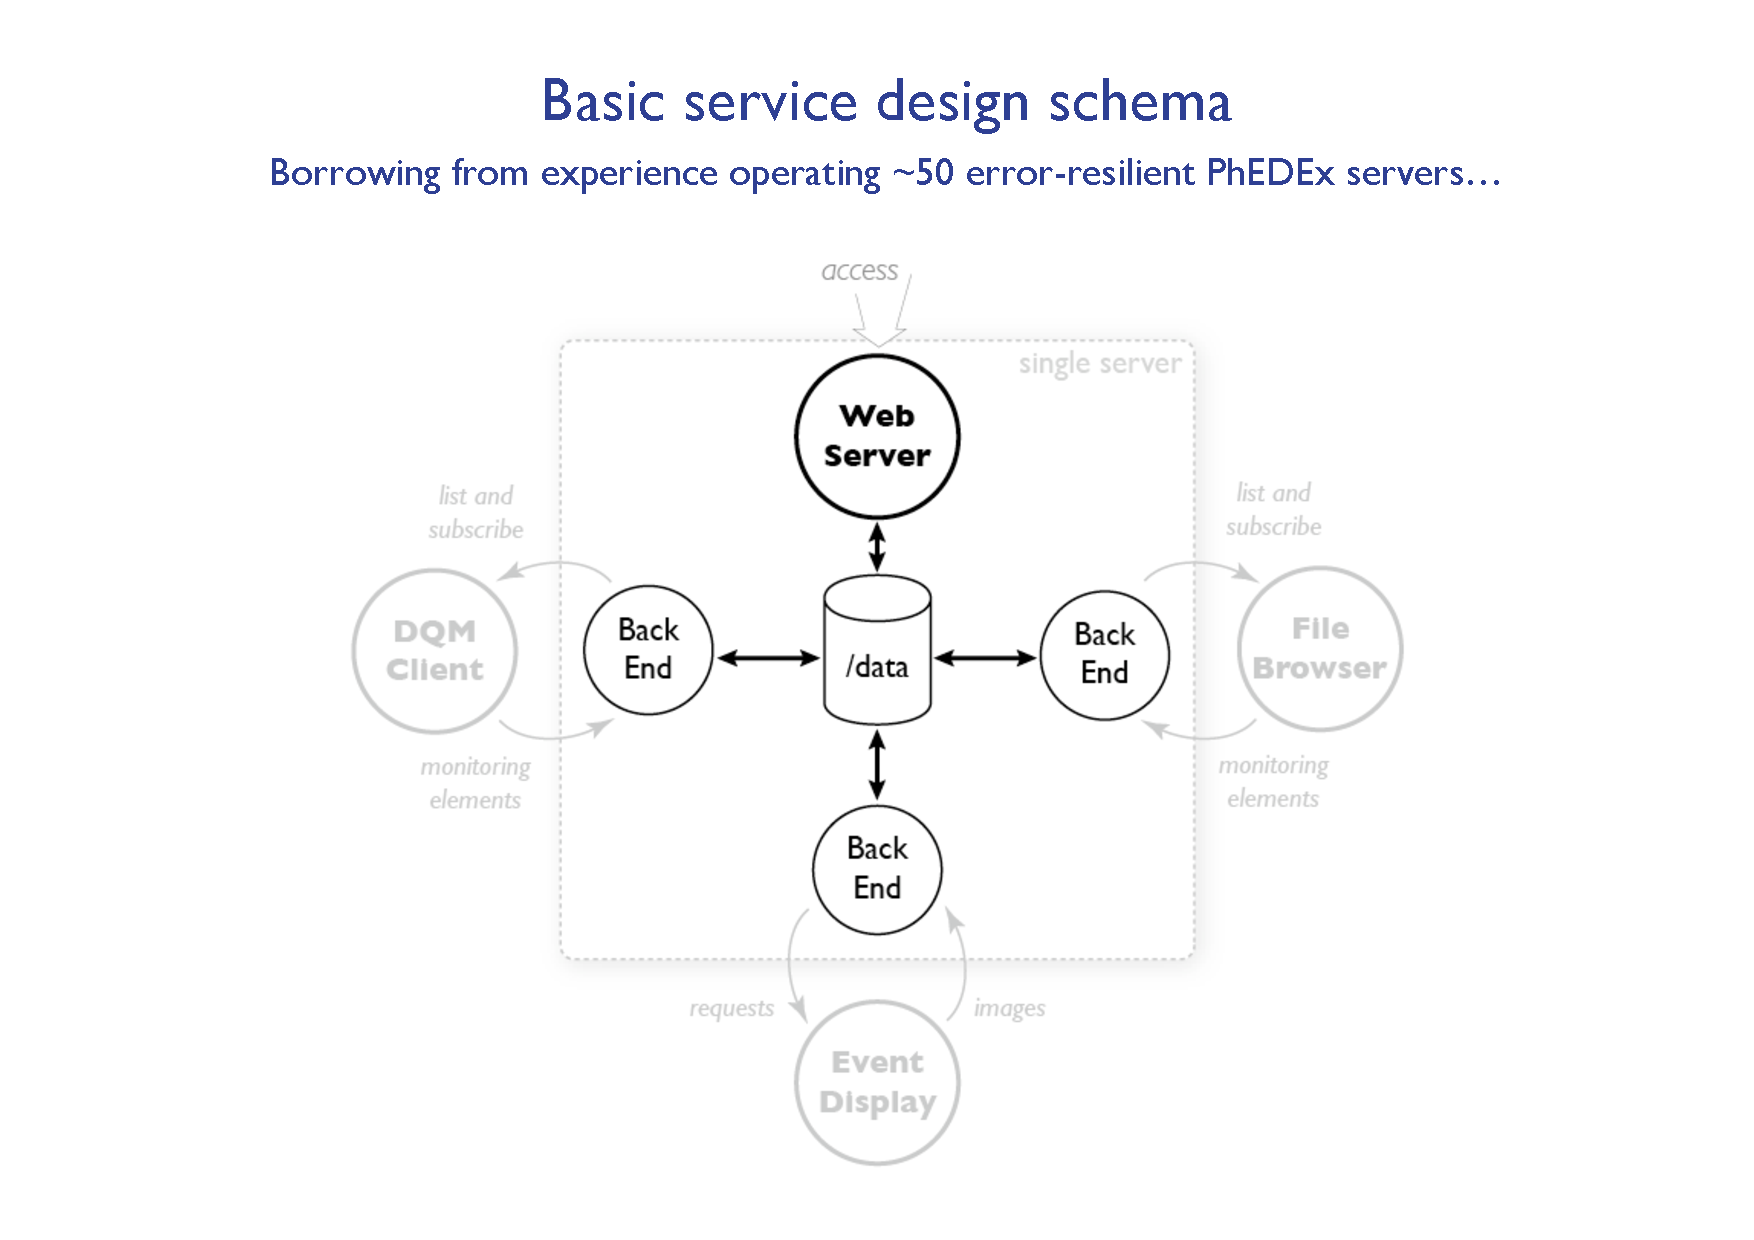
\includegraphics[width=0.9\textwidth]{GUI}
\caption{Webserver based DQM Visualization with different backend
for access to online DQM as well as output from offline processing
(figure taken from \cite{talk:lassi}). }
\end{center}
\label{fig:gui}
\end{figure}

\subsection{Requirements}

\begin{itemize}
\item Histogram collection, rendering and display
\begin{itemize}       
   \item The GUI collects DQM information from all possible sources, possibly including subsystem-based DQM facilities as well as results from XDAQ based DAQ monitoring. 
   \item Up to 12 histograms are displayed at once at any given time. 
   \item A summary display is provided that indicates available information, e.g. the current situation of subscriptions and histogram updates.
\end{itemize}
\item Histogram Navigation and Decoration 
\begin{itemize}
\item The same webserver GUI provides switches between different backends (e.g. live-online, online from file-archive, offline etc).
\item Operation modes, such as expert and shift, remote and P5, online and offline are configurable.
\item For online DQM a detector component based directory structure is used, reflecting the several subsystem-dependent sources.
\item A number of histogram views are foreseen, based on different aspects such as synoptic views (e.g. for shift operation), as well as detailed views based on geometrical position, frontend and cabling map, alarm state etc. In addition a search functionality (based on the histogram name is foreseen).
\item Individual layouts simplify retrieval of user-specified views making lengthy repetitive navigation obsolete. A slide show mode will be useful for the purpose of shift-browsing.
\item Subsystems can provide display plug-ins which specify the way histograms are rendered (colour-palettes and decorations etc.)
\item A facility for overlaying reference histograms is in place.
\item Customizable menus for histogram decoration (e.g. depending on quality test results) and labeling (including instructions to non-expert users (shift) about possible features that are significant of error states) are provided.
\item Facilities for histogram zooming and pointering are in place.
\item In order to display distributions of single LS a subtraction facility is foreseen, in which accumulated data from two subsequent LS are subtracted to retrieve the distributions of one single LS.
\item For navigation and interactivity aspects a webserver public interface is being considered. This way javascript components which conform with this interface can be collected in a library and attached to the GUI on demand.
\item Online DQM functionality beyond that implemented in iguana, e.g.\,components of the well-advanced implementation of DQM visualization tools based on XDAQ by the silicon and strip tracker groups is going to be realized. 
\item Visualization of live history and trends %CHECK
\item Full development, deployment of the error collector
and integration with offline data certification.
\item Assembly of static run-wise summary webpages (`page-1 of DQM')
\end{itemize}
\end{itemize}

\subsection{Online Summary Views}
\label{sec:summary}

The purpose of online DQM being prompt and efficient identification of problems, the most prominant goal of online Monitoring must be to distribute all relevant information quickly to where ever it is needed.

Each online DQM sub-system will provide three pieces of DQM summary information:
\begin{itemize}
\item the reportSummary ME (type: float) containing a global summary of the detector state
\item the reportSummaryMap ME (type: TH2F) containing a 2d histogram with report information as function of eta - phi.
\item the reportSummarySegments folder, containing a collection of MonitorElements of type float which are used to describe the behavior of sub-sub-system components. This collection of floats allows the sub-system to provide useful information about their inner/low-level state.
\end{itemize}
All three kinds of objects are under the sub-system responsibility, both booking and filling (the DQMEventInfo will be cleaned up).

This information is displayed in the following way:
\begin{itemize}
\item the EventInfo/reportSummary float ME will remain in the top table in the Summary workspace. this table is the only one shown by default.
\item by clicking on the 'sub-system' name in the table (in on/off fashion), the empty space below the table will show:
\begin{itemize}
\item on the left side the EventInfo/reportSummaryMap TH2D MEs
\item on the right side, a table (two columns, several rows) showing the list of the float MEs contained in EventInfo/reportSummarySegments, with their names and values (in the future we expect the names to change according to the sub-sytem needs, without changes in the GUI).
\end{itemize}
\end{itemize}

\subsection{Interactivity}

Interactivity is constrained to navigating through the list of available DQM results and visualizing them. In addition it is foreseen that users can modify the sensitivity of the display to alarm states by changing specific histogram decorations and sound-levels.

However, there will be no real-time interaction between the user (e.g. subsystem expert) and DQM-client applications. DQM applications can be configured to perform any activity required at the beginning of each run. In addition stand-alone DQM applications that receive events from the same Storage Manager event server can be launched at any time. 

%==========================================================
% this subsection is common to all sections, please fill in
\subsection{DQM GUI System Integration and Operation}

\subsubsection*{Integration}
\subsubsection*{Operation}
